\chapter{Loogiset lauseet}

Logiikkaa ja erilaisia päättelyitä käytetään jatkuvasti arkipäivän tilanteissa. Logiikan tutkimuksessa tarvitaan kuitenkin täsmällisiä mää\-ri\-tel\-miä ja systemaattisia päättelysääntöjä, joihin tutustutaan tässä luvussa.

\section{Atomilauseet, konnektiivit ja totuusarvot}
\label{konnektiivit}

\subsection*{Tutkimustehtävä}
Neljä opiskelijaa hakee kesätöihin huvipuistoon. Tutustu heidän hakutietoihinsa. Vastaa kysymyksiin hakijoiden soveltuvuudesta eri tehtäviin.

Hanna (17 v.) on opiskellut kaksi vuotta ammattilukiossa. Opintoihinsa liittyen hän on suorittanut hygieniapassin. Hanna harrastaa tennistä ja kalliokiipeilyä.

Heikki (18 v.) on opiskellut kaksi vuotta lukiossa. Hänellä on ajokortti ja hygieniapassi. Heikki pelkää korkeita paikkoja.

Jussi (18 v.) on opiskellut yhden vuoden lukiossa ja on juuri palannut Uudesta-Seelannista, missä hän oli vaihto-opiskelijana yhdeksän kuukautta.

Saara (19 v.) on suorittanut ylioppilastutkinnon. Hän kirjoitti mm. pitkän englannin ja lyhyen ranskan. Saara on ollut vuoden vaihto-opiskelijana Englannissa, ja hänellä on ajokortti.

\begin{enumerate}
\item Jarrumieheksi vuoristoradalle voidaan valita henkilö, joka ei pelkää korkeita paikkoja. Sopiiko a) Hanna b) Heikki teh\-tä\-vään?
\item Oppaalta vaaditaan lukion pitkän englannin oppimäärä tai yli puolen vuoden oleskelu englanninkielisessä maassa. Sopiiko a) Jussi b) Saara c) Hanna tehtävään?
\item Jäätelökärryn kuljettajalta vaaditaan täysi-ikäisyyttä ja hygieniapassia. Sopiiko a) Saara b) Hanna c) Heikki tehtävään?
\end{enumerate}

\bigskip

\begin{center}
\includegraphics[width=6cm]{pictures/kuvitus/Rollercoaster\vari}
\end{center}

\bigskip

Yksinkertaisimpia loogisia lauseita kutsutaan \termi{atomilause}{atomilauseiksi}. Atomilauseita käytetään ilmaisemaan asioiden tilaa. Esimeriksi seuraavat lauseet ovat atomilauseita:
\begin{enumerate}[$A:$]
\item On yö.
\item Aurinko paistaa.
\item Pariisi on Italiassa.
\item Oulu on Suomessa.
\end{enumerate}
Atomilauseita ajatellaan eräänlaisina totuusmuuttujina, jotka voivat saada kaksi arvoa: tosi tai epätosi. Yllä olevista lauseista $C$ on epätosi, $D$ on tosi ja kaksi ensimmäistä voivat olla tosia tai epätosia ajankohdasta riippuen. Tässä kurssissa atomilauseita merkitään isoilla kirjaimilla $A$, $B$, $C$, jne. Todelle ja epätodelle käytetään tietotekniikasta tuttuja merkintöjä $1$ ja $0$.

Loogisia lauseita voidaan myös muodostaa yhdistelemällä atomilauseita \termi{konnektiivi}{konnektiivien} avulla. Konnektiiveja ovat esimerkiksi \termi{ei}{ei}, \termi{ja}{ja}, \termi{tai}{tai} sekä \termi{jos ... niin}{jos ... niin}. Näillä sanoilla on myös arkikielessä merkityksiä, jotka joskus eivät täysin vastaa niiden merkitystä logiikassa. Lausetta, jossa on vähintään yksi konnektiivi, kutsutaan \termi{yhdistetty lause}{yhdistetyksi lauseeksi}. Yhdistetyn lauseen totuusarvoa tutkitaan \termi{totuustaulu}{totuustaulujen} avulla.

\subsection*{Negaatio} Yksinkertaisin esimerkki konnektiivista on looginen ei, jota kutsutaan \termi{negaatio}{negaatioksi}. Lauseen $A$ negaatiota merkitään $\lnot A$. Negaation totuusarvo on vastakkainen sille lauseelle, johon negaatio liittyy. Jos $A$ on tosi, niin $\lnot A$ on epätosi. Jos $A$ on epätosi, niin $\lnot A$ on tosi.

Esimerkiksi lauseen $A$: ''uimahalli on auki'' negaatio on $\lnot A$: ''uimahalli on suljettu''.

%Logiikassa on tapana esittää rakenteita \termi{totuustaulu}{totuustaulun} avulla. 
Negaation totuustaulu on seuraava:

%\bigskip

\bigskip

\begin{center}
\begin{tabular}{|c|c|}\hline
$A$ & $A$:n negaatio \\ \hline
tosi & epätosi \\ 
epätosi & tosi \\
\hline
\end{tabular}
\end{center}

\bigskip

Aikaisemmin mainittuja merkintöjä käyttäen totuustaulu voidaan kirjoittaa lyhyemmin:

\bigskip

\begin{center}
\begin{tabular}{|c|c|}\hline
$A$ & $\lnot A$ \\ \hline
$1$ & $0$\\ 
$0$ & $1$ \\ \hline
\end{tabular}
\end{center}

\bigskip

\subsection*{Konjunktio}
Loogista ja-konnektiivia sanotaan \termi{konjunktio}{konjunktioksi}. Kahden lauseen $A$ ja $B$ konjunktio $A\land B$ on tosi vain silloin, kun molemmat kyseisistä lauseista ovat tosia. Muussa tapauksessa se on epätosi.

Esimerkiksi lauseiden $A$: ''olen vaaleatukkainen'' ja $B$: ''olen ruskeasilmäinen'' konjunktio on $A \land B$: ''olen vaaleatukkainen ja ruskeasilmäinen''. 

Konjunktion totuustaulu:

\bigskip

\begin{center}
\begin{tabular}{|c|c|c|}\hline
$A$ & $B$ & $A\land B$ \\ \hline
$1$ & $1$ & $1$\\ 
$1$ & $0$ & $0$\\
$0$ & $1$ & $0$\\
$0$ & $0$ & $0$\\
\hline
\end{tabular}
\end{center}

\bigskip

\subsection*{Disjunktio} Loogista tai-konnektiivia sanotaan \termi{disjunktio}{disjunktioksi}. Lauseiden $A$ ja $B$ disjunktio $A\lor B$ on tosi silloin, kun ainakin toinen lauseista $A$ ja $B$ on tosi.


Esimerkiksi lauseiden $A$: ''henkilöllä on B-ajokortti'' ja $B$: ''henkilöllä on moottoripyöräkortti'' disjunktio on $A \lor B$: ''henkilöllä on B-ajokortti tai hänellä on moottoripyöräkortti''. 

Disjunktion totuustaulu:
 
\bigskip

\begin{center}
\begin{tabular}{|c|c|c|}\hline
$A$ & $B$ & $A\lor B$ \\ \hline
$1$ & $1$ & $1$\\ 
$1$ & $0$ & $1$\\
$0$ & $1$ & $1$\\
$0$ & $0$ & $0$\\ \hline
\end{tabular}
\end{center}

\bigskip

Kannattaa huomata, että arkikielessä sanalla tai on usein eri merkitys kuin logiikassa, koska tai-lauseen ei aina ajatella olevan tosi tapauksessa, jossa sekä $A$ että $B$ ovat tosia.

Esimerkiksi hampurilaisateriaan voi valita ranskalaiset perunat tai minisalaatin mutta ei molempia. Toisaalta henkilö on vapaa oppivelvollisuudesta, jos hänellä on peruskoulun päästötodistus tai jos koulun aloittamisesta on kulunut kymmenen vuotta. Kumpi tahansa ehto yksinään riittää. Suurimmalla osalla oppivelvollisuudesta vapaista ihmisistä on kummatkin ominaisuudet.

%{\bf Esimerkki 1.}
\begin{esimerkki}
Olkoot lauseet $A$: ''on kesä'', $B$: ''käyn töissä'' ja $C$: ''pelaan jalkapalloliigassa''. Suomenna lauseet
\begin{enumerate}[a)]
\item $\lnot A$, 
\item $B\lor C$,
\item $\lnot A\land B$,
\item $B\lor (A\land C)$.
\end{enumerate}

{\bf Ratkaisu:}
\begin{enumerate}[a)]
\item Ei ole kesä.
\item Käyn töissä tai pelaan jalkapalloliigassa.
\item Ei ole kesä ja käyn töissä.
\item Käyn töissä, tai sitten on kesä ja pelaan jalkapalloliigassa.
\end{enumerate}
\end{esimerkki}


\subsection*{Formalisointi}
\termi{formalisointi}{Formalisoinnilla} tarkoitetaan luonnollisen kielen, esimerkiksi suomen kielen, lauseiden kääntämistä logiikan kielelle. Tällöin on esimerkiksi valittava, mitkä ovat atomilauseita. Samalla ilmaisulla voi olla useita mielekkäitä formalisointeja. Formalisoinnin tarkoituksena on löytää vastaavuuksia logiikan ja arkielämän tilanteiden välille. Näin voidaan esimerkiksi tutkia erilaisia väitelauseita ja päätelmiä. Formalisointi on tärkeä väline eräiden filosofian ja tietojenkäsittelyn ongelmien tutkimuksessa.

Arkikielen lauseiden kääntäminen logiikan kielelle ei ole aina helppoa ja tulkinnanvaraisuuttakin voi esiintyä. Erityisen ongelmallisia ovat paljon konnektiiveja sisältävät lauseet, koska luonnollisessa kielessä konnektiivien suoritusjärjestystä ei määritellä eikä tavallisesti käytetä sulkeita.

\begin{esimerkki}
%{\bf Esimerkki 2.}  
Formalisoi lauseet
\begin{enumerate}[a)]
\item Liisalla ei ole alibia. 
\item Liisalla on alibi tai hänellä ei ole motiivia.
\item Liisalla on motiivi, mutta hänellä on myös alibi.
\item Alibin puuttuessa Liisalla ei ole motiivia. 
\end{enumerate}

{\bf Ratkaisu:}
Käytetään atomilauseita $A$: ''Liisalla on alibi'' ja $M$: ''Liisalla on motiivi''.	
Formalisoidut lauseet ovat:
\begin{enumerate}[a)]
\item $\lnot A$.
\item $A \lor \lnot M$.
\item $M\land A$.
\item Lause voidaan ymmärtää niin, että Liisalla ei ole alibia eikä hänellä myöskään ole motiivia. Silloin sen formalisointi on $\lnot A \land \lnot M$. Toisaalta lause voidaan tulkita niin, että alibin puuttumisesta seuraa se, että Liisalla ei ole motiivia. Tätä lausetta ei ole suoraviivaista formalisoida negaation, konjunktion ja disjunktion avulla. Siihen tarvitaan niiden lisäksi seuraavassa kappaleessa esiteltävä implikaatio. 
\end{enumerate}

{\bf Vastaus:}
a) $\lnot A$, b) $A \lor \lnot M$, c) $M\land A$, d) esimerkiksi 
$\lnot A \land \lnot M$.
\end{esimerkki}

%{\bf Esimerkki 3.}
\begin{esimerkki}
Lomamatkallaan Liina ja Pasi halusivat osallistua rullaluistelutapahtumaan. He  näkivät tarjouksen: ''Vuokraa 5 eurolla rullaluistimet tai suojat ja kypärä!'' Miten tarjous pitäisi ymmärtää?

{\bf Ratkaisu:}
Tarjous ei ole yksiselitteinen. Käytetään atomilauseita $R$: ''vuokraan kuuluu rullaluistimet'', $S$: ''vuokraan kuuluu suojat'' ja $K$: ''vuokraan kuuluu kypärä''. Tarjous olisi formalisoituna $R\lor S \land K$. Lauseen merkitys riippuu kuitenkin siitä, kumpaa	konnektiivia sovelletaan ensin. Lause $R\lor (S\land K)$ tarkoittaa, että viidellä eurolla voi vuokrata joko pelkästään rullaluistimet tai sitten sekä suojat että kypärän. Lause $(R\lor S)\land K$ tarkoittaa, että viidellä eurolla voi vuokrata joko rullaluistimet tai suojat ja niiden lisäksi kypärän. 

{\bf Vastaus:} Tarjouksen voi ymmärtää kahdella tavalla:
viidellä eurolla voi vuokrata joko pelkästään rullaluistimet tai sitten sekä suojat että kypärän; viidellä eurolla voi vuokrata joko rullaluistimet tai suojat ja niiden lisäksi kypärän.
\end{esimerkki}

Formalisoinnin jälkeen lauseen totuusarvoa voidaan tutkia esimerkiksi totuustaulujen avulla.

%{\bf Esimerkki 4.}
\begin{esimerkki}
Laadi totuustaulu lauseelle a) $\lnot(A\land \lnot B)$, b) $(A\land B)\lor \lnot C$.

{\bf Ratkaisu:}
\begin{enumerate}[a)]
\item Lauseessa $\lnot(A\land \lnot B)$ on kaksi atomilausetta. Totuustauluun merkitään kaikki lauseiden $A$ ja $B$ eri totuusarvojen yhdistelmät. Sen jälkeen kirjoitetaan sarakkeet lauseiden $\lnot B$, $A\land \lnot B$ sekä $\lnot(A\land \lnot B)$  totuusarvoille.
\bigskip

\begin{center}
\begin{tabular}{|c|c|c|c|c|}\hline
$A$ & $B$ & $\lnot B$ & $A\land \lnot B$ & $\lnot(A\land \lnot B)$ \\ \hline
$1$ & $1$ & $0$       & $0$ & $1$ \\ 
$1$ & $0$ & $1$       & $1$ & $0$ \\
$0$ & $1$ & $0$       & $0$ & $1$ \\
$0$ & $0$ & $1$       & $0$ & $1$ \\ \hline
\end{tabular}
\end{center}

\bigskip

\item Lauseessa $(A\land B)\lor \lnot C$ on kolme atomilausetta. Kaikkia lauseiden $A$, $B$ ja $C$ totuusarvojen yhdistelmiä varten tarvitaan kahdeksan riviä.

\bigskip

\begin{center}
\begin{tabular}{|c|c|c|c|c|c|}\hline
$A$ & $B$ & $C$ & $\lnot C$ & $A\land B$ & $(A\land B)\lor \lnot C$\\ \hline
$1$ & $1$ & $1$ & $0$ & $1$ & $1$ \\ %\hline
$1$ & $1$ & $0$ & $1$ & $1$ & $1$ \\
$1$ & $0$ & $1$ & $0$ & $0$ & $0$ \\
$1$ & $0$ & $0$ & $1$ & $0$ & $1$ \\
$0$ & $1$ & $1$ & $0$ & $0$ & $0$ \\
$0$ & $1$ & $0$ & $1$ & $0$ & $1$ \\
$0$ & $0$ & $1$ & $0$ & $0$ & $0$ \\
$0$ & $0$ & $0$ & $1$ & $0$ & $1$ \\ \hline
\end{tabular}
\end{center}

\end{enumerate}
\end{esimerkki}

\Harjoitustehtavat

\begin{enumerate}
\item Onko lause atomilause?
a) Tampere on Pirkanmaalla. b) Kajaani on Suomen pääkaupunki. c) Hattu pois päästä! d) On olemassa suurin alkuluku.
e) Onko avaruudessa elämää? f) $5 + 12 = 18$.

\item Kirjoita lauseen negaatio.
\begin{enumerate}[a)]
\item Tänään on maanantai.
\item $2+3=5$.
\item Luku on negatiivinen.
\item Ainakin yhdellä ryhmämme opiskelijalla on ruskeat silmät.
\item Kymmenessä sivussa tekstiä on vähintään seitsemän virhettä.
\item Kesä Välimerellä on kuuma ja aurinkoinen.
\end{enumerate}

\item Olkoot lause $A$: ''veikkasin lottorivin'' ja lause $B$: ''voitin miljoona euroa''. Kirjoita suomen kielellä lauseet
a) $\lnot A$, b) $A\lor B$, c) $A\land B$, d) $A\land \lnot B$,  
e) $\lnot A\lor (A\land B)$, f) $\lnot A\land \lnot B$.

\item
Olkoot lause $A$: ''on kaunis kesäpäivä'',  lause $B$: ''lokit kirkuvat'' ja lause $C$: ''kävelen rannalla''. Kirjoita suomen kielellä lauseet
a) $\lnot A\lor B$,
b) $A\land B \land C$, c)
$\lnot(A\land C)$,
d) $(A\land C)\lor (B\land
\lnot C)$.

\item Olkoot $A$: ''on pilvistä'' ja $B$: ''sataa
lunta''. Formalisoi seuraavat lauseet eli kirjoita ne
lauseiden $A$ ja $B$ sekä konnektiivien $\lnot$, $\land$
ja $\lor$ avulla.
\begin{enumerate}[a)]
\item On pilvistä ja sataa lunta.
\item On pilvistä, mutta ei sada lunta.
\item Ei ole pilvistä eikä sada lunta.
\item On pilvistä tai sataa lunta.
\item On pilvistä ja sataa lunta tai ei ole pilvistä
eikä sada lunta.
\end{enumerate}

\item Formalisoi lauseet:
\begin{enumerate}[a)]
\item Mustikat polun varrella ovat kypsiä tai
alueella ei ole nähty karhuja.
\item Ei ole totta, että mustikat polun varrella ovat
kypsiä tai alueella on nähty karhuja.
\item Mustikat polun varrella ovat kypsiä, mutta
alueella ei ole nähty karhuja, tai sitten mustikat eivät
ole kypsiä ja alueella on nähty karhuja.
\item Karhuja ei ole nähty alueella ja polulla
vaeltaminen on turvallista, mutta mustikat ovat kypsiä.
\end{enumerate}

\item
\begin{enumerate}[a)]
\item Laadi totuustaulu lauseelle $\lnot A\lor \lnot
B$. Millä atomilauseiden $A$ ja $B$ totuusarvoilla lause
on tosi?
\item Laadi totuustaulu lauseelle $\lnot(A\land B)$.
Millä atomilauseiden $A$ ja $B$ totuusarvoilla lause on
tosi? Vertaa a-kohdan tulokseen.
\item Keksi atomilauseet $A$ ja $B$ ja ilmaise a- ja
b-kohtien lauseet suomen kielellä.
\end{enumerate}

\item Laadi totuustaulu lauseelle $(A\land B)\lor \lnot (B\lor C)$.

\item Olkoot atomilauseet $A$: ''$x < -1$'', $B$: ''$x > 1$''  ja $C$: ''$x = 1$''. Formalisoi  lauseet  
a)  $x\neq 1$,   b) $x \ge 1$,   c)  $x \ge -1$,  d)  $x < 1$,  e)  $-1 \le x \le  1$, 
f) $x <  -1$ tai $x  \ge 1$.        

\item
Saarella asuu haltijoita ja menninkäisiä. Turisti tapasi kaksi saarelaista, Hipsun ja Vipsun. Hipsu sanoi: ''Hillat ovat kypsiä ja kalaonni on suotuisa, tai sitten hillat eivät ole kypsiä tai kalaonni ei ole suotuisa.'' Vipsu väitti: ''Hillat ovat kypsiä ja kalaonni on suotuisa, mutta hillat eivät ole kypsiä tai kalaonni ei ole suotuisa.'' Tutki totuustaulun avulla Hipsun ja Vipsun väitteiden totuusarvoja. Mitä voidaan päätellä totuustaulun avulla, kun tiedetään, että saaren asukkaista haltijat valehtelevat aina ja menninkäiset puhuvat aina totta? Saiko vierailija käyttökelpoista tietoa marjasadosta tai kalaonnesta?


%\end{enumerate}

%\newpage

%\section*{Loogiset piirit}
\item
Loogisilla piireillä suoritetaan digitaalisissa laitteissa erilaisia loogisia operaatioita. Loogisen piirin toimintaa voidaan kuvata esimerkiksi seuraavalla kaaviolla.

\medskip

\begin{center}
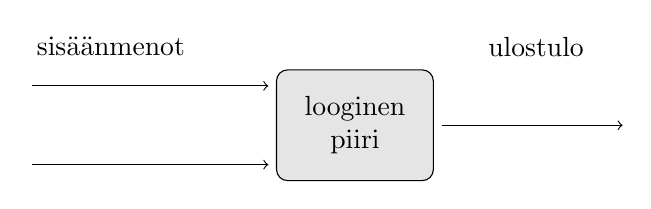
\begin{tikzpicture}
\node [rectangle, draw, fill=gray!20, text width=5em, text centered, rounded corners, minimum height=4em] at (4.1,1) {looginen piiri};
\draw [->] (0,0.5) -- (3,0.5);
\draw [->] (0,1.5) -- (3,1.5);
\draw [->] (5.2,1) -- (7.5,1);


\node at (1,2) {sisäänmenot};
\node at (6.4,2) {ulostulo};
\end{tikzpicture}
\end{center}

\medskip

Loogisella piirillä on yksi tai useampi sisäänmeno ja
yksi tai useampi ulostulo. Tämän kirjan esimerkeissä ja
tehtävissä käsitellään vain yhden ulostulon piirejä.
Sisäänmenojen ja ulostulon signaalin arvo
voi olla 1 tai 0. Edellisessä tapauksessa johtimessa on
jännite, jälkimmäisessä tapauksessa ei ole.

Loogiset piirit kootaan loogisista porteista. Seuraavassa
taulukossa on lueteltu loogiset portit, niiden toiminta
ja toimintaa vastaava looginen konnektiivi.

%\newpage

\small

\begin{center}
\begin{tabular}{|>{\centering}m{1.5cm}|>{\raggedright}m{3.8cm}|c|>{\centering\arraybackslash}m{2cm}|}
\hline
Looginen portti & \centering Toiminta & Piirrosmerkki & Looginen konnektiivi \\
% \begin{tabular}{c}
% %Toimintaa \\
% %	vastaava \\
% Looginen \\
% konnektiivi
% \end{tabular}
\hline

Tai &
Tai-portti antaa jännitteen, kun ainakin toisessa sisäänmenossa on jännite. &

%\begin{center}
\raisebox{-.5\height}{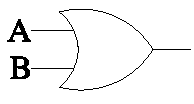
\includegraphics[width=2.5cm]{pictures/boole/or-ABC}}
%\end{center}
&
$A\lor B$
\\ \hline

Ja &
Ja-portti antaa jännitteen vain silloin, kun molemmissa sisäänmenoissa on jännite. &

%\begin{center}
\raisebox{-.5\height}{
\includegraphics[width=2.5cm]{pictures/boole/and-ABC}}
%\end{center}
&
$A\land B$
\\ \hline

Ei &
Ei-portti antaa jännitteen silloin, kun sisäänmenossa ei ole jännitettä, ja kääntäen. &
%\begin{center}
\raisebox{-.5\height}{
\includegraphics[width=2.5cm]{pictures/boole/not-ABC}}
%\end{center}
&
$\lnot A$
\\ \hline

\end{tabular}

\end{center}

\normalsize

%\newpage

\bigskip

Esimerkiksi looginen piiri

\medskip

\begin{center}
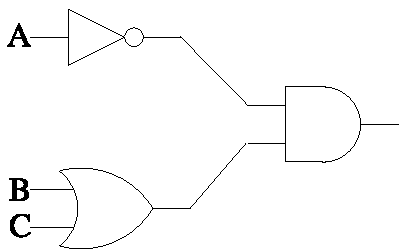
\includegraphics[width=3.5cm]{pictures/boole/boolesim-ABC}
\end{center}

\medskip
\noindent
koostuu kolmesta loogisesta portista ja vastaa
lausetta \mbox{$\lnot A\lor (B \land C)$}.

%{\bf Tehtäviä}

%\begin{enumerate}
Muodosta seuraavia piirejä vastaavat lauseet.

a)
\begin{center}
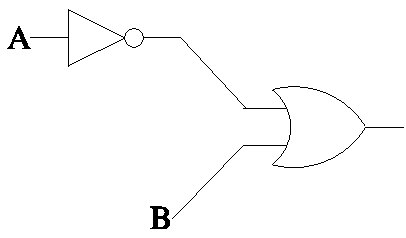
\includegraphics[width=3.5cm]{pictures/boole/boolt-a-ABC}
\end{center}

b)
\begin{center}
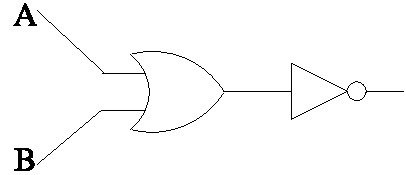
\includegraphics[width=3.5cm]{pictures/boole/boolt-b-ABC}
\end{center}

c)
\begin{center}
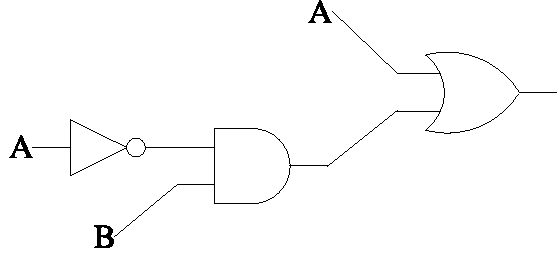
\includegraphics[width=4cm]{pictures/boole/boolt-c-ABC}
\end{center}

d)
\begin{center}
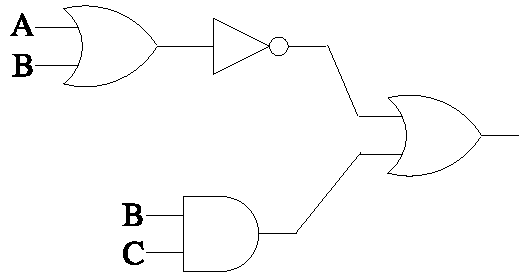
\includegraphics[width=4.5cm]{pictures/boole/boolt-d-ABC}
\end{center}

\item
Piirrä lausetta
a) $\lnot A \land B$ b) $A\lor \lnot (B\land C)$ c)
$(A\land B)\lor (\lnot A \land C)$
vastaava looginen piiri.

\end{enumerate}

\subsection*{Kotitehtäviä}

\begin{enumerate}

\item  Kirjoita lauseen negaatio.
\begin{enumerate}[a)]
\item $100 > 101$.
\item Lompakossani on rahaa korkeintaan 10 euroa.
\item Kaikki ryhmämme opiskelijat ovat Facebookissa.
\item Koulussamme on täsmälleen kaksi vasenkätistä opettajaa.
\item En opiskele latinaa enkä kreikkaa.
\item Maarit pitää lumilautailusta tai käsitöistä muttei molemmista.
\end{enumerate}

\item Olkoot lauseet $A$: ''puutarhan portti on auki'', $B$: ''ruusut kukkivat'' ja $C$: ''menen puutarhaan''. Kirjoita suomen kielellä lauseet a) $\lnot A$,  b)  $B\land C$,  c)  $A\lor B$,
d) $\lnot B \land \lnot C$,  e)  $\lnot(A\land B)$  f)  $A \lor \lnot B$,   g)  $(A \land C) \lor (\lnot B \land C)$. 

\item Formalisoi lause.
\begin{enumerate}[a)]
\item Kaino ei ole vanha ja Kaino on mies.
\item Kaino on vanha tai Kaino ei ole mies.
\item Kaino ei ole vanha mies. 
\item Kaino ei ole vanha eikä hän ole mies.
\end{enumerate}

\item Formalisoi lause.
\begin{enumerate}[a)]
\item Amadeus kuuntelee klassista tai Klaus kuuntelee jazzia.
\item Amadeus ei kuuntele klassista, mutta Klaus kuuntelee jazzia.
\item Amadeus kuuntelee klassista, mutta Klaus ei kuuntele jazzia, tai sitten Hassinen kuuntelee progea.
\item Ei ole niin, että Amadeus kuuntelisi klassista, Klaus jazzia ja Hassinen progea.
\end{enumerate}

\item 
\begin{enumerate}[a)]
\item Laadi totuustaulu lauseille $A\land \lnot A$ ja $A\lor \lnot A$.
\item Keksi atomilause $A$ ja ilmaise kohdan a) lauseet suomen kielellä.
\end{enumerate}

\item
Laadi totuustaulu lauseille a) $\lnot(A\lor B)$,  b)  $\lnot A\land B$,  c) $ (\lnot A\lor B)\land (A\lor \lnot B)$. Millä atomilauseiden $A$ ja  $B$ totuusarvojen yhdistelmillä lauseet ovat tosia?

\item
\begin{enumerate}[a)]
\item Laadi totuustaulu lauseelle $A\lor (B\land C)$.  
\item Laadi totuustaulu lauseelle $(A\lor B)\land C$. 
\item Vertaa kohtien a) ja b) lauseiden totuusarvoja. Mitä voit päätellä?
\end{enumerate}

\item Olkoot lauseet $A$: ''$x\in [-3,1]$'' ja $B$: ''$ x \in [-1,5]$''. Formalisoi lause.
a) $x\in [-3,5]$, b) $x\in [-1,1]$,   c)  $x\in [-3,-1[$  d)  $x\in ]-\infty,-3[$  tai $x\in ]1,\infty[$, 
e) $x\in]-\infty,-3[$  tai $x\in ]5,\infty[$.  

\item Kolme koiranpentua, Alli, Buh ja Caesar ovat epäiltyinä isännän tohvelin repimisestä. Luotettava henkilö, joka puhuu aina totta, antaa seuraavan todistuksen: ''Ei ole totta, että Alli on syyllinen tai Buh ei ole syyllinen. Mutta kuitenkin Alli on syyllinen tai Caesar on syyllinen.'' Käytä atomilauseita $A$: ''Alli on syyllinen'', $B$: ''Buh on syyllinen'' ja $C$: ''Caesar on syyllinen'' ja formalisoi luotettavan henkilön lausunto. Muodosta sille totuustaulu ja päättele, mikä tai mitkä koiranpennuista ovat syyllisiä. 

\item Tutkitaan lausetta ''Suomen kuningas ei ole viiksekäs''. Lause voidaan tulkita ainakin kahdella eri tavalla:
\begin{enumerate}[a)]
\item Suomella on kuningas, joka ei ole viiksekäs.
\item Ei ole niin, että olisi olemassa Suomen viiksekästä kuningasta.
\end{enumerate}
Oletetaan, että Suomessa ei ole kuningasta. Onko lause tosi vai epätosi?

\item
Kissoilla lyhyen karvan aiheuttaa dominoiva geeni ja pitkän karvan resessiivinen geeni. Merkitään lyhyen karvan geeniä S ja pitkän karvan geeniä s. Kaikilla nisäkkäillä tiettyyn ominaisuuteen vaikuttaa geenipari, joista toinen geeni on saatu isältä ja toinen emolta. Jos kissan geeneistä ainakin toinen on S, niin se on lyhytkarvainen. Kissa on pitkäkarvainen vain siinä tapauksessa, että se on saanut geenin s molemmilta vanhemmiltaan.  Pentujen emokissa on pitkäkarvainen (ss) ja isäkissa lyhytkarvainen (SS tai Ss). Millaisia pentuja kissat voivat saada, kun isäkissan geenipari on a) SS b) Ss?

\end{enumerate}

%\newpage


\section{Implikaatio ja ekvivalenssi}
Tässä kappaleessa esitellään kaksi usein käytettyä konnektiivia: \termi{implikaatio}{implikaatio} eli \termi{looginen seuraus}{looginen seuraus} sekä \termi{ekvivalenssi}{ekvivalenssi} eli \termi{looginen yhtäpitävyys}{looginen yhtäpitävyys}.

\subsection*{Tutkimustehtävä}

\begin{center}
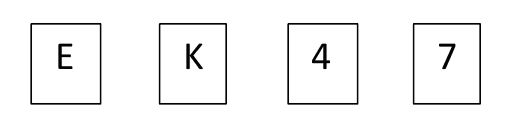
\includegraphics[width=7cm]{pictures/piaget}
\end{center}

Tarkastellaan oheisen kuvan mukaisia kortteja. Korttien toisella puolella on jokin kirjain ja toisella puolella jokin luku.

1) Ongelmana on selvittää, toteuttavatko kortit seuraavan säännön: Jos kortin toisella puolella on vokaali, niin sen toisella puolella on parillinen luku. Mitkä kortit täytyy vähintään kääntää?

2) Ongelmana on selvittää, toteuttavatko kortit seuraavan säännön: Kortin toisella puolella on parillinen luku, jos ja vain jos sen toisella puolella on vokaali. Mitkä kortit täytyy vähintään kääntää?

Psykologi Jean Piaget\footnote{\url{http://webspace.ship.edu/cgboer/piaget.html}} (1896 -- 1980) käytti ensimmäistä kysymystä tutkiessaan nuorten ja aikuisten abstraktia ajattelua.

\subsection*{Implikaatio}

Loogista jos $A$ niin $B$ -rakennetta sanotaan implikaatioksi. Implikaatiota merkitään $A\to B$. Implikaatiota  kutsutaan toisinaan loogiseksi seu\-rauk\-sek\-si, mutta tämä ilmaisu on hieman tulkinnanvarainen. Sanalla seuraus on nimittäin puhekielessä kaksi sanan loogisesta merkityksestä poikkeavaa mutta tavallisempaa merkitystä. Seuraus voi tarkoittaa esimerkiksi ajallista seurausta, eli asia tapahtuu toisen jälkeen. Sanalla voidaan myös tarkoittaa kausaalista seurausta, eli asia on toisen aiheuttava syy. Logiikassa ei yleensä kiinnitetä huomiota tällaisiin näkökohtiin. Joskus asiat voivat olla toistensa loogisia seurauksia, vaikka niillä ei olisi kausaalisesti mitään tekemistä toistensa kanssa. Esimerkiksi lause ''jos Caesar elää, niin Helsinki sijaitsee Afrikassa'' on logiikan mielessä tosi. 

%\laatikko{
Looginen implikaatio $A\to B$  määritellään niin, että se on epätosi ainoastaan tapauksessa, jossa $A$ on tosi mutta $B$ ei ole. Kaikissa muissa tapauksissa se on tosi. Siksi logiikassa usein sanotaan, että epätodesta oletuksesta voi päätellä mitä tahansa.


Esimerkiksi lauseista $A$: ''Anne on suomalainen'' ja $B$: ''Anne on eurooppalainen'' saadaan implikaation avulla lauseet $A \to B$: ''jos Anne on suomalainen, niin hän on eurooppalainen'' sekä myös $B \to A$: ''jos Anne on eurooppalainen, niin hän on suomalainen''. 

Implikaation totuustaulu:

\bigskip

\begin{center}
\begin{tabular}{|c|c|c|}\hline
$A$ & $B$ & $A \to B$ \\ \hline
$1$ & $1$ & $1$\\ %\hline
$1$ & $0$ & $0$\\
$0$ & $1$ & $1$\\
$0$ & $0$ & $1$\\ \hline
\end{tabular}
\end{center}

\bigskip

Kappaleessa \ref{monimloog} osoitetaan, että implikaatiota voidaan ajatella lyhennysmerkintänä lauseelle $\lnot A \lor B$, koska implikaatiolla on sama totuustaulu kuin kyseisellä lauseella.


\subsection*{Ekvivalenssi}
Jos sekä $A\to B$ että $B\to A$ ovat tosia lauseita, sanotaan, että lauseet $A$ ja $B$ ovat ekvivalentit, $A \lequiv B$. Ekvivalenssia voi ajatella lyhennysmerkintänä lauseelle $(A\to B) \land (B\to A)$. Intuitiivisesti se tarkoittaa lauseiden $A$ ja $B$ yhtäpitävyyttä (vrt. yhtäsuuruus), eli molemmat lauseet saavat samat totuusarvot.


Esimerkiksi lauseiden $A$: ''Pekka menee hammaslääkäriin'' ja $B$: ''Pekan hammasta särkee'' ekvivalenssi on $A \lequiv B$: ''Pekka menee hammaslääkäriin, jos ja vain jos hänen hammastaan särkee''.

Ekvivalenssin totuustaulu:

\bigskip

\begin{center}
\begin{tabular}{|c|c|c|}\hline
$A$ & $B$ & $A \lequiv  B$ \\ \hline
$1$ & $1$ & $1$\\ %\hline
$1$ & $0$ & $0$\\
$0$ & $1$ & $0$\\
$0$ & $0$ & $1$\\ \hline
\end{tabular}
\end{center}

\bigskip

Ekvivalenssi $A\lequiv B$ voidaan lukea ''$A$, jos ja vain jos $B$''. Tämä ilmaisu esiintyy usein matemaattisessa tekstissä. Voidaan käyttää myös esimerkiksi ilmaisuja ''$A$ silloin ja vain silloin, kun $B$'' ja ''$A$ ja $B$ ovat yhtäpitävät''.


\begin{esimerkki}
%{\bf Esimerkki 1.}
Formalisoi lause. Missä tilanteissa lause on tosi? a) On kesä, ja jos on kesä, järvivesi on lämmintä. b) Uin silloin ja vain silloin, kun on kesä ja järvivesi on lämmintä. 

{\bf Ratkaisu:}
Käytetään atomilauseita $A$: ''on kesä'',
$B$: ''järvivesi on lämmintä'' ja $C$: ''uin''.
\begin{enumerate}[a)]
\item Lause on $A \land (A \to B)$. Muodostetaan
lauseen totuustaulu.

\bigskip

\begin{center}
\begin{tabular}{|c|c|c|c|}\hline
$A$ & $B$ & $A \to B$ & $A \land (A \to B)$\\ \hline
$1$ & $1$ & $1$ & $1$\\ %\hline
$1$ & $0$ & $0$ & $0$\\
$0$ & $1$ & $1$ & $0$\\
$0$ & $0$ & $1$ & $0$\\ \hline
\end{tabular}
\end{center}

\bigskip

Lause on tosi täsmälleen silloin, kun $A$ ja $B$ ovat
molemmat tosia eli kun on kesä ja järvivesi on lämmintä.
\item Lause on $C \lequiv (A \land B)$. Muodostetaan
lauseen totuustaulu.

\bigskip

\begin{center}
\begin{tabular}{|c|c|c|c|c|c|}\hline
$A$ & $B$ & $C$ & $A \land B$ & $C \lequiv (A \land B)$\\
\hline
$1$ & $1$ & $1$ & $1$ & $1$\\ %\hline
$1$ & $1$ & $0$ & $1$ & $0$\\
$1$ & $0$ & $1$ & $0$ & $0$\\ %\hline
$1$ & $0$ & $0$ & $0$ & $1$\\
$0$ & $1$ & $1$ & $0$ & $0$\\
$0$ & $1$ & $0$ & $0$ & $1$\\ %\hline
$0$ & $0$ & $1$ & $0$ & $0$\\
$0$ & $0$ & $0$ & $0$ & $1$\\ \hline
\end{tabular}
\end{center}

\bigskip

Lause on tosi, kun atomilauseet $A$, $B$ ja $C$ ovat
kaikki tosia, kun $A$ on tosi sekä $B$ ja $C$ ovat
epätosia, kun $B$ on tosi sekä $A$ ja $C$ ovat epätosia
tai kun kaikki atomilauseet ovat epätosia. Tämä vastaa
seuraavia tilanteita: on kesä, järvivesi on lämmintä ja
uin; on kesä, järvivesi ei ole lämmintä enkä ui; ei ole
kesä, järvivesi on lämmintä, mutta en ui; ei ole kesä,
järvivesi ei ole lämmintä enkä ui.
\end{enumerate}

{\bf Vastaus: } a) Lause on tosi, kun on kesä ja järvivesi on lämmintä.

b) Lause on tosi seuraavissa tilanteissa: on kesä, järvivesi on lämmintä 
ja uin; on kesä, järvivesi ei ole lämmintä enkä ui; ei ole 
kesä, järvivesi on lämmintä, mutta en ui; ei ole kesä, 
järvivesi ei ole lämmintä enkä ui.
\end{esimerkki}

%{\bf Esimerkki 2.}
\begin{esimerkki}
Matti, Seppo ja Teppo ovat epäiltyinä rikoksesta. Heitä kuulusteleva konstaapeli Reinikainen tietää, että syytön puhuu aina totta ja syyllinen valehtelee aina.

Matti sanoi: ''Jos Seppo on syytön, niin minäkin olen.''

Seppo väitti: ''Minä olen syytön, jos ja vain jos Teppo on syytön.''

Teppo sanoi: ''Seppo yksin on syyllinen.'' 

Ratkaise totuustaulun avulla, kuka tai ketkä ovat syyllisiä.

{\bf Ratkaisu:} Tarkastellaan lauseita $M$: ''Matti on syytön'', $S$: ''Seppo on syytön'' ja $T$: ''Teppo on syytön''.

Matin, Sepon ja Tepon väitteet formalisoituina ovat $S\to M$, $S\lequiv T$
ja $M\land \lnot S \land T$. Tutkitaan, kuinka väitteet riippuvat lauseiden $M$, $S$ ja $T$ totuusarvoista. Muodostetaan totuustaulu:

\bigskip

\begin{center}
\begin{tabular}{|c|c|c|c|c|c|c|c|}\hline
$M$ & $S$ & $T$ & $S\to M$ & $S\lequiv T$ & $\lnot S$ & $M\land \lnot S$ & $M\land \lnot S \land T$\\ \hline
$1$ & $1$ & $1$ & $1$ & $1$ & $0$ & $0$ & $0$\\ %\hline
$1$ & $1$ & $0$ & $1$ & $0$ & $0$ & $0$ & $0$\\
$1$ & $0$ & $1$ & $1$ & $0$ & $1$ & $1$ & $1$\\
$1$ & $0$ & $0$ & $1$ & $1$ & $1$ & $1$ & $0$\\
$0$ & $1$ & $1$ & $0$ & $1$ & $0$ & $0$ & $0$\\
$0$ & $1$ & $0$ & $0$ & $0$ & $0$ & $0$ & $0$\\
$0$ & $0$ & $1$ & $1$ & $0$ & $1$ & $0$ & $0$\\
$0$ & $0$ & $0$ & $1$ & $1$ & $1$ & $0$ & $0$ \\ \hline
\end{tabular}
\end{center}

\bigskip

Koska syytön puhuu totta ja syyllinen valehtelee, on löydettävä totuustaulusta rivi, jolla väitteillä $S\to M$, $S\lequiv T$ ja $M \land \lnot S\land T$ on samat totuusarvot kuin lauseilla $M$, $S$ ja $T$. Tällainen rivi on totuustaulun kolmas rivi. Siten Seppo on yksin syyllinen.

{\bf Vastaus:} Seppo on yksin syyllinen.
\end{esimerkki}

\bigskip

\subsection*{Konnektiivien suoritusjärjestys} 
Loogisten lauseiden lukeminen helpottuu ja tarve sulkeiden käyttämiseen vähenee, jos sovitaan konnektiivien suoritusjärjestyksestä. Nykyään yleisimmin käytetään seuraavaa suoritusjärjestystä, jota noudatetaan myös tässä kirjassa: $\lnot$, $\land$, $\lor$, $\to$, $\lequiv$, ja vasemmalta oikealle.

Suoritusjärjestystä voidaan muuttaa käyttämällä sulkeita. Sulkeita kannattaa myös käyttää aina silloin, kun se helpottaa loogisen lauseen lukemista.

%{\bf Esimerkki 3.}
\begin{esimerkki}
Mikä on lauseiden a) $B \lequiv \lnot A\lor B \land A \to B$, ja  b)  $(B\lequiv \lnot A)\lor B \land (A\to B)$  totuusarvo, kun $A$ on tosi ja $B$ epätosi?   

{\bf Ratkaisu:}

%\begin{enumerate}[a)]
%\item

a) Muodostetaan totuustaulu:

\begin{footnotesize}
\begin{center}
\begin{tabular}{|c|c|c|c|c|c|c|}\hline
$A$ & $B$ & $\lnot A$ & $B \land A $ & $\lnot A\lor B \land A$ & $\lnot A\lor B \land A \to B$ & $B \lequiv \lnot A\lor B \land A \to B$\\ \hline
$1$ & $0$ & $0$ & $0$ & $0$ & $1$ & $0$\\ \hline
\end{tabular}
\end{center}
\end{footnotesize}

Ensin suoritetaan negaatio. Sen jälkeen tulevat konjunktio ja disjunktio. Implikaatio 	suoritetaan ennen ekvivalenssia. 	Kun $A$ on tosi ja $B$ epätosi, lause on epätosi.

%\item

b) Muodostetaan totuustaulu:

\begin{footnotesize}
\begin{center}
\begin{tabular}{|c|c|c|c|c|c|c|}\hline
$A$ & $B$ & $\lnot A$ & $B\lequiv \lnot A$ & $A\to B$ & $B \land (A\to B)$ &  $(B\lequiv \lnot A)\lor B \land (A\to B)$\\ \hline
$1$ & $0$ & $0$ & $1$ & $0$ & $0$ & $1$\\ \hline
\end{tabular}
\end{center}
\end{footnotesize}

Ensin suoritetaan negaatio. Sen jälkeen tulevat sulkeissa olevat ekvivalenssi ja implikaatio. Konjunktio suoritetaan ennen disjunktiota. Kun $A$ on tosi ja $B$ epätosi, lause on tosi.

{\bf Vastaus:} a) epätosi, b) tosi
\end{esimerkki}

\subsection*{Harvinaisempia konnektiiveja}% (Lisämateriaalia).}
Logiikassa ja tietotekniikassa esiintyy myös muita, harvinaisempia loogisia konnektiiveja. Esimerkki tällaisesta on \termi{poissulkeva tai}{poissulkeva tai} (engl. exclusive or), josta usein käytetään tietotekniikasta tulevaa lyhennettä \termi{xor}{xor}. Poissulkevan tain totuustaulu on seuraava:

\bigskip

\begin{center}
\begin{tabular}{|c|c|c|}\hline
$A$ & $B$ & $A\,\mathrm{xor}\,B$ \\ \hline
$1$ & $1$ & $0$\\ %\hline
$1$ & $0$ & $1$\\
$0$ & $1$ & $1$\\
$0$ & $0$ & $0$\\ \hline
\end{tabular}
\end{center}

\bigskip

Kuten kappaleessa \ref{konnektiivit} todettiin, arkikielessä sana tai saattaa tarkoittaa asiayhteydestä riippuen joskus poissulkevaa tai-operaatiota ja toisinaan loogista disjunktiota.

Lisää loogisia konnektiiveja esitellään harjoitustehtävissä.


%\newpage

%\bigskip

%\section*{Tehtäviä}
\Harjoitustehtavat

\begin{enumerate}
\item Olkoot $A$: ''Matti on insinööri'' ja $B$: ''Matilla on hyvä työpaikka''.
Suomenna lause.
\begin{enumerate}[a)]
\item $A\land B$,
\item $\lnot A \lor B$,
\item $A\to B$,
\item $\lnot B\to A$,
\item $\lnot( B \to A )$.
\item $ B \lequiv A$.
\end{enumerate}

\item Olkoot $A$: ''Liisa on lomalla'' ja $B$: ''Liisa on iloinen''. Formalisoi lauseet:
\begin{enumerate}[a)]
\item Jos Liisa on lomalla, hän on iloinen.
\item Liisa on lomalla, mutta hän ei ole iloinen.
\item Liisa on iloinen silloin ja vain silloin, kun hän on lomalla.
\item Jos Liisa ei ole iloinen, hän ei ole lomalla.
\end{enumerate}

\item Onko lause tosi?
\begin{enumerate}[a)]
\item Jos Tallinna on Norjan pääkaupunki, niin Tukholma on Ruotsin pääkaupunki.
\item Jos Tallinna on Norjan pääkaupunki, niin Budapest on Ruotsin pääkaupunki.
\item Jos Leonardo da Vinci on kuollut, niin Aleksis Kivi on saksalainen ralliautoilija.
\item Jos Leonardo da Vinci on kuollut, niin Leo Tolstoi on venäläinen kirjailija.
\end{enumerate}

\item Laadi lauseen totuustaulu.
\begin{enumerate}[a)]
\item $\lnot A \to B$
\item $A\lequiv \lnot B$
\item $\lnot( A\land B )\to A$
\end{enumerate}

\item Laadi lauseen totuustaulu.
\begin{enumerate}[a)]
\item $\lnot A \lor B \to C \land A$
\item $( A\to B ) \lequiv (C\to B)$
\end{enumerate}

\item Formalisoi lause. Missä tilanteissa lause on tosi?
\begin{enumerate}[a)]
\item
Jos mustikat polun varrella eivät ole kypsiä, niin polulla vaeltaminen on turvallista.
\item Jos mustikat polun varrella ovat kypsiä, niin silloin polulla vaeltaminen on turvallista, jos ja vain jos karhuja ei ole nähty alueella. 
\item Polulla vaeltaminen on turvallista silloin ja vain silloin, kun mustikat eivät ole kypsiä tai alueella ei ole nähty karhuja.
\end{enumerate}

\item Formalisoi lause ja laadi lauseen totuustaulu. Mitä huomaat? Kertooko lause mitään siitä, onko logiikan opiskelu oikeasti hauskaa juuri tällä hetkellä? 
\begin{enumerate}[a)]
\item Jos sataa ja ei sada, niin logiikan opiskelu on hauskaa.
\item Jos sataa ja ei sada, niin logiikan opiskelu ei ole hauskaa.
\end{enumerate}

\item Perheen lapsia Annaa ja Markusta epäillään kaappiin piilotetun suklaalevyn katoamisesta. Luotettava todistaja kertoo tiedot:
Anna on syyllinen tai Markus on syyllinen.
Anna on syytön tai Markus on syytön. 
Jos Anna on syyllinen, niin Markus on syyllinen.

Kumpi lapsista on käynyt suklaavarkaissa?

\item Edwards, Petterson ja Smith ovat syytettyinä omenavarkaudesta. Neiti Marble kuulustelee heitä. Edwards sanoo: ''Jos Petterson on syytön, niin minä olen syyllinen.'' Petterson toteaa: ''Minä olen syyllinen, jos ja vain jos Edwards on syyllinen.'' Smith väittää: ''Olemme kaikki syyttömiä.'' Neiti Marble tietää, että syylliset valehtelevat aina ja syyttömät puhuvat aina totta. Ratkaise totuustaulun avulla, kuka tai ketkä syytetyistä ovat käyneet omenavarkaissa.

\item Eräässä maassa kaikki kuuluvat joko hattujen tai myssyjen puolueeseen. Hatut valehtelevat aina ja myssyt puhuvat aina totta. Kolme kansalaista keskusteli keskenään. Heidän joukossaan saattoi olla vieraan puolueen vakoilija. Arthur sanoi, että Claus on myssy. Berit totesi, että Arthur on myssy ja myös hän itse on myssy. Claus väitti, että jos Arthur on hattu, niin myös hän itse on hattu. Tutki totuustaulun avulla, kuka oli mahdollinen vakoilija.

\item Olkoot lauseet $A$: ''herään ajoissa'', $B$: ''menen kouluun'' ja $C$: ''opiskelen logiikkaa''.
Esitä sanoin lause $A \to B \lor C$. Onko lauseen tulkinta $A \to (B \lor C)$ vai $(A \to B) \lor C$? Miten tulkinnat eroavat toisistaan? 

\item
Vertaa lauseiden totuusarvoja atomilauseiden $A$, $B$ ja $C$ eri totuusarvoilla. Onko sulkeiden muuttamisella vaikutusta lauseen totuusarvoon?
\begin{enumerate}[a)]
\item $(A\to B)\to C$ ja $A\to (B\to C)$.
\item $(A\land B)\land C$ ja $A\land (B\land C)$.
\end{enumerate}

\item (Lisämateriaalia)  Tietokoneet käsittelevät tietoa käyttäen bittejä. Bitillä on kaksi mahdollista arvoa, $0$ ja $1$.
Bittijono on jono, jossa on yksi tai useampia bittejä. Esimerkiksi $1001\, 0010$ on bittijono, jonka pituus on $8$ bittiä. Samanpituisille bittijonoille määritellään bittikohtaiset tai, ja sekä poissulkeva tai (or, and sekä xor). Esimerkiksi bittijonojen $1100$ ja $1010$ bittikohtainen tai on jono $1110$, bittikohtainen ja on jono $1000$ sekä bittikohtainen poissulkeva tai on jono $0110$. Muodosta a) bittikohtainen tai  b) bittikohtainen ja c) bittikohtainen poissulkeva tai jonoille $1111\, 0000$ ja $1010\, 1010$.

\item (Lisämateriaalia)  Muodosta bittijono a)  $(0\, 1111 \land 1\, 0101) \lor 0\, 1000$  b) $(0\, 1010 \xor 1\, 1011) \xor 0\, 1001$. 

\end{enumerate}

\subsection*{Kotitehtäviä}

\begin{enumerate}

\item
Olkoot $A$: ''Timo opiskelee matematiikkaa'', $B$: ''Timo osallistuu logiikan kurssille'' ja $C$: ''Timo opiskelee filosofiaa''. Suomenna lause.
\begin{enumerate}[a)]
\item $\lnot A \to \lnot B$.
\item $A\lequiv B$.
\item $A\lor C \to B$.
\item $C\lequiv (B\to \lnot A)$.
\end{enumerate}

\item Onko lause tosi?
\begin{enumerate}[a)]
\item Jos $(-2)^3= -8$, niin $(-2)^3= -8$.
\item Jos $(-2)^3= -8$, niin $(-2)^3=  8$.
\item Jos luku $8$ on pariton, niin luku $8$ on pariton.
\item Jos luku $8$ on pariton, niin luku $8$ on parillinen.
\end{enumerate}

\item
Formalisoi lause.
\begin{enumerate}[a)]
\item Jos opettaja on pirteä, niin televisiosta ei ole tullut illalla jalkapalloa.
\item Suomi voittaa jalkapallon maailmanmestaruuden silloin ja vain silloin, kun lehmät lentävät ja vaaleanpunaiset norsut kävelevät kadulla.
\item En seuraa jalkapalloa eikä Suomen maajoukkue menesty. 
\item Jos ottelu ei pääty tasapeliin, niin joko kotijoukkue tai vierasjoukkue voittaa pelin.
\end{enumerate}

\item Laadi lauseen totuustaulu.
\begin{enumerate}[a)]
\item $A\land B\to \lnot B$
\item $(A\lequiv B)\land B\to C\lor A$
\item $(\lnot A\to B)\lequiv (C\to B\land A)$
\end{enumerate}


\item
Olkoot $A$: ''Timo opiskelee matematiikkaa'', $B$: ''Timo osallistuu logiikan kurssille'' ja $C$: ''Timo opiskelee filosofiaa''. Formalisoi lause. Missä tilanteissa lause on tosi?
\begin{enumerate}[a)]
\item Timo opiskelee matematiikkaa ja filosofiaa.
\item Jos Timo opiskelee matematiikkaa, hän osallistuu logiikan kurssille.
\item Timo osallistuu logiikan kurssille silloin ja vain silloin, kun hän opiskelee filosofiaa tai matematiikkaa.
\item Jos Timo osallistuu logiikan kurssille, opiskelee hän joko matematiikka tai filosofiaa, muttei molempia.
\end{enumerate}

\bigskip

\begin{center}
\includegraphics[width=8cm]{pictures/kuvitus/Finnish_police_car\vari}
\end{center}

\item Poliisit Mauno ja Martti saavat kiinni rikoksesta epäilemänsä Jaskan. Tiedetään, että Jaska ei koskaan valehtele. Mauno toteaa Martille: ''Jos Jaska on syyllinen, on hänellä ollut rikostoveri.'' Jaska vastaa: ''Tuo ei ole totta!'' Tähän Martti tokaisee: ''Sehän tunnusti helpolla!'' Tutki Maunon lausetta ja osoita Martin johtopäätös oikeaksi.

\item Mattia, Seppoa ja Teppoa epäillään polkupyörävarkaudesta. Konstaapeli Reinikainen tietää, että syytön puhuu aina totta ja syyllinen valehtelee aina. Reinikainen kuulustelee kolmea epäiltyä. Matti sanoo: ''Teppo on syyllinen.'' Seppo väittää: ''Matti on syyllinen tai Teppo valehtelee.'' Teppo toteaa: ''Seppo on syyllinen.'' Ratkaise totuustaulun avulla, kuka on syyllinen. 

\item Helinä, Heljä ja Helena asuvat samassa talossa. Epäillään, että loton päävoitto on osunut taloon. Luotettavalta taholta on tullut tietoja:

Jos Heljä on voittaja, niin Helinäkin on. 
Heljä on voittaja, jos ja vain jos Helena on voittaja.
Ainakin yksi naisista on voittaja, mutta kaikki eivät ole.

Kuka tai ketkä ovat voittaneet lotossa?

\item
Mitä eroa on seuraavissa ehdoissa?
\begin{enumerate}
\item Henkilö saa työpaikan matkamuistomyymälässä, jos hänellä on kokemusta kassakoneen käytöstä.
\item Matkamuistomyymälässä työskentelevältä edellytetään kokemusta kassakoneen käytöstä.
\item 
Henkilö saa työpaikan matkamuistomyymälässä silloin ja vain silloin, kun hänellä on kokemusta kassakoneen käytöstä.
\end{enumerate}


\item
Vertaa lauseiden totuusarvoja atomilauseiden $A$, $B$ ja $C$ eri totuusarvoilla. Onko sulkeiden muuttamisella vaikutusta lauseen totuusarvoon?

\begin{enumerate}[a)]

\item $(A\lor B)\lor C$ ja $A\lor (B\lor C)$.

\item $(A\lequiv B)\lequiv C$ ja $A\lequiv (B\lequiv C)$.

\item $\lnot A \lequiv (B \land C)$ ja $\lnot (A \lequiv B) \land C$.

\end{enumerate}

%\item Muodosta
%\begin{enumerate}[a)]
%\item lauseen $A$ ja lauseen $B$ negaation konjunktio,
%\item lauseiden $A$ ja $B$ disjunktion negaatio,
%\item lauseen $A$ negaation ekvivalenssi lauseiden $B$ ja $C$ konjunktion kanssa.
%\end{enumerate}

\item
Olkoon $v$ sellainen funktio, että $v(A) = 1$, jos lause $A$ on tosi, ja $v(A) = 0$, jos lause $A$ on epätosi. Osoita, että yhtälö pätee kaikilla lauseiden $A$ ja $B$ totuusarvojen yhdistelmillä.

\begin{enumerate}[a)]
\item $v(A\land B)=v(A)v(B)$,
\item $v(A\lor B)=v(A)+v(B)- v(A)v(B)$,
\item $v(A\to B)=1-v(A)(1-v(B))$.
\end{enumerate}

\item
Peircen nuoli on konnektiivi, joka luonnollisessa kielessä tarkoittaa samaa kuin ''ei $A$ eikä $B$''. Shefferin viiva on konnektiivi, joka luonnollisessa kielessä tarkoittaa samaa kuin ''ei molemmat $A$ ja $B$''. Laadi näiden konnektiivien totuustaulut. 
\end{enumerate}

\newpage

\section{Monimutkaisempia loogisia rakenteita}
\label{monimloog}
Seuraavaksi tarkastellaan eräitä usein esiintyviä loogisia rakenteita. Tällaisia rakenteita ovat \termi{tautologia}{tautologiat}, \termi{loogisesti ekvivalentti lause}{loogisesti ekvivalentit} ja \termi{ristiriitainen lause}{ristiriitaiset lauseet}. On tärkeää oppia tunnistamaan nämä rakenteet, koska niitä käytetään usein logiikan yhteydessä.

\subsection*{Tutkimustehtävä}
Turisti tapasi kaksi saarelaista, Hipsun ja Vipsun. Hän kyseli heiltä, kuinka hyvin kala syö, ja sai seuraavat vastaukset.
\begin{enumerate}
\item On pilvistä, tai sitten jos kala ei syö, niin ei ole pilvistä.
\item On pilvistä tai kala syö, mutta ei ole pilvistä eikä kala syö.
\end{enumerate}
Formalisoi lauseet käyttäen atomilauseita $P$: ''on pilvistä'' ja $K$: ''kala syö''. Tutki totuustaulun avulla, milloin väitteet ovat tosia. Mitä huomaat?

\subsection*{Tautologia}
Tautologialla tarkoitetaan lausetta, joka on tosi riippumatta asioiden tilasta. Tällainen lause on esimerkiksi: ''Huominen on aina tulevaisuutta.'' Sanaa tautologia käytetään filosofiassa myös argumenteista, joita ei voi kumota tekemättä ristiriitaisia oletuksia.

\begin{esimerkki}
%{\bf Esimerkki 1.} 
Osoita, että lause $(A\land B)\lor (\lnot A \lor \lnot B)$ on
tautologia.

{\bf Ratkaisu:}
Muodostetaan lauseen $(A\land B)\lor (\lnot A \lor \lnot
B)$ totuustaulu:

\begin{center}
\begin{tabular}{|c|c|c|c|c|c|c|}\hline
$A$ & $B$ & $A\land B$ & $\lnot A$ & $\lnot B$ & $ \lnot
A \lor \lnot B $ & $(A\land B)\lor (\lnot A \lor \lnot B)$
\\ \hline
$1$ & $1$ & $1$ & $0$ & $0$ & $0$ & $1$ \\ %\hline
$1$ & $0$ & $0$ & $0$ & $1$ & $1$ & $1$ \\
$0$ & $1$ & $0$ & $1$ & $0$ & $1$ & $1$ \\
$0$ & $0$ & $0$ & $1$ & $1$ & $1$ & $1$ \\ \hline
\end{tabular}
\end{center}

Koska lause on aina tosi, se on tautologia.
\end{esimerkki}

\subsection*{Looginen ekvivalenssi}  Loogisesti
ekvivalentit lauseet saavat samat totuusarvot
kaikissa tilanteissa. Kaksi lausetta $L_1$ ja
$L_2$ ovat siis  loogisesti ekvivalentteja, jos niillä
on samat totuustaulut. Toisin sanoen lause $L_1 \lequiv L_2$ on tautologia.

\begin{esimerkki}
%{\bf Esimerkki 2.}
 Osoita, että lauseet $A\to B$ ja $\lnot A \lor B$ ovat loogisesti
ekvivalentit.

{\bf Ratkaisu:}
Verrataan lauseiden $A\to B$ ja $\lnot A \lor B$
totuustauluja: 

\begin{center}
\begin{tabular}{|c|c|c|c|c|}\hline
$A$ & $B$ & $A\to B$ & $\lnot A$ & $\lnot A\lor B$ \\ \hline
$1$ & $1$ & $1$ & $0$ & $1$  \\ %\hline
$1$ & $0$ & $0$ & $0$ & $0$  \\
$0$ & $1$ & $1$ & $1$ & $1$  \\
$0$ & $0$ & $1$ & $1$ & $1$  \\ \hline
\end{tabular}
\end{center}

Koska lauseiden $A\to B$ ja $\lnot A \lor B$ totuusarvot
ovat aina samat, lauseet ovat loogisesti ekvivalentit.
\end{esimerkki}

\termi{kolmannen poissulkevan laki}{Kolmannen poissulkevan laki} sanoo, että kaikki lauseet ovat joko tosia tai epätosia. Formaalilla kielellä kolmannen poissulkevan laki tarkoittaa, että lause $A \lor \lnot A$ on tautologia. Tämä voidaan nähdä seuraavasta totuustaulusta:

\bigskip

\begin{center}
\begin{tabular}{|c|c|c|}\hline
$A$ & $\lnot A$ & $A \lor  \lnot A$ \\ \hline
$1$ & $0$ & $1$\\
$0$ & $1$ & $1$\\ \hline
\end{tabular}
\end{center}

\bigskip


\subsection*{Moniarvoiset logiikat}% (lisämateriaalia).}
Lauseen $A \lor \lnot A$ tautologisuus liittyy klassisen logiikan kaksiarvoisuuteen. Voidaan ajatella myös sellaisia päättelymalleja, joissa lause $A \lor \lnot A$ ei ole tautologia. Esimerkki tällaisesta on \termi{kolmiarvoinen logiikka}{kolmiarvoinen logiikka}, jossa mahdollisia totuusarvoja ovat tosi, epätosi ja epävarma.  Toinen esimerkki on niin kutsuttu \termi{sumean logiikka}{sumean logiikka}, jossa on äärettömän monta totuusarvoa. Erilaiset päättelyjärjestelmät eivät kuitenkaan kumoa toisiaan, vaan logiikkaa sovellettaessa käytetään kuhunkin tilanteeseen sopivaa päättelyjärjestelmää. Esimerkiksi kolmiarvoinen logiikka soveltuu tilanteisiin, joissa käytössä oleva informaatio ajatellaan epätäydelliseksi.


\subsection*{Ristiriitainen lause}
Lausetta, joka ei toteudu missään tilanteessa, kutsutaan loogisesti ristiriitaiseksi. Lauseen ristiriitaisuutta voidaan jälleen tutkia totuustaulun avulla. Loogisesti ristiriitaisen lauseen negaatio on tautologia. 

Yksinkertaisin esimerkki ristiriitaisesta lauseesta on lause $A\land \lnot A$. Sen totuustaulu on seuraava:

\bigskip

\begin{center}
\begin{tabular}{|c|c|c|}\hline
$A$ & $\lnot A$ & $A \land  \lnot A$ \\ \hline
$1$ & $0$ & $0$\\
$0$ & $1$ & $0$\\ \hline
\end{tabular}
\end{center}

\bigskip


\subsection*{Päättelysääntöjä} Logiikassa esiintyy monia hyödyllisiksi havaittuja päättelysääntöjä, joille on annettu nimi. Nämä päättelysäännöt ovat esimerkkejä tautologioista, ja niiden tautologisuus voidaan osoittaa esimerkiksi totuustaulua käyttämällä.

Tärkeitä päättelysääntöjä ovat esimerkiksi \termi{De Morganin lait}{De Morganin lait}
\[
\lnot(A \land B) \lequiv \lnot A \lor \lnot B
\]
ja
\[
\lnot(A \lor B) \lequiv \lnot A \land \lnot B,
\]
jotka liittävät toisiinsa loogiset ja- sekä tai-konnektiivit.
%{\bf de Morganin lait.}

\termi{kaksoisnegaation laki}{Kaksoisnegaation laki} sanoo, että lauseen $A$ kaksinkertainen negaatio $\lnot \lnot A$ on loogisesti ekvivalentti lauseen $A$ kanssa:
\[
\lnot \lnot A \lequiv A.
\]
\termi{kontraposition laki}{Kontraposition laki} puolestaan sanoo, että lauseet $A\to B$ ja $\lnot B \to \lnot A$ ovat loogisesti ekvivalentit. Tämän voi osoittaa paitsi totuustauluja käyttämällä myös soveltamalla De Morganin lakeja.
Matematiikassa tärkeä todistusmenetelmä, niin sanottu käänteinen todistus, perustuu kontraposition lakiin. Käänteistä todistusta käsitellään luvussa 4.

%	{\bf Laita perustelu esimerkiksi. Myös mieti mahdollista viittausta käänteiseen todistukseen (Antti/AM).}
%kk(käytä muotoilua lauseet ... ovat loogisesti ekvivalentit).

Seuraavaan taulukkoon on koottu edellisten lisäksi muutamia muita tunnetuimpia päättelysääntöjä: %***********

\bigskip

\laatikko{
%\begin{center}
\begin{tabular}{|l|c|}
\hline
{\bf Päättelysääntöjä} & \\\hline
\termi{De Morganin 1. laki}{De Morganin 1. laki} & $\lnot(A \land B) \lequiv \lnot A \lor \lnot B$\\\hline
\termi{De Morganin 2. laki}{De Morganin 2. laki} & $\lnot(A \lor B) \lequiv \lnot A \land \lnot B$\\\hline
\termi{Kaksoisnegaation laki}{Kaksoisnegaation laki} & $\lnot \lnot A \lequiv A$\\\hline
\termi{Kontraposition laki}{Kontraposition laki} & $(A\to B)\lequiv (\lnot B \to \lnot A)$\\\hline
\termi{Modus ponens}{Modus ponens} & $(A\land (A\to B)) \to B$ \\\hline
\termi{Modus tollens}{Modus tollens} & $((A\to B) \land \lnot B) \to \lnot A$ \\\hline
\termi{Reductio ad absurdum}{Reductio ad absurdum} & $(\lnot A \to (B \land \lnot B))\to A$\\\hline
\end{tabular}
%\end{center}
}

\bigskip

%{\bf Esimerkki 3.}
\begin{esimerkki}
Esitä  sanallinen muotoilu a) De Morganin 1. laille
\[
\lnot (A\land B) \lequiv \lnot A \lor \lnot B,
\]
b) modus tollens -päättelysäännölle
\[
((A\to B)\land \lnot B) \to \lnot A.
\]

{\bf Ratkaisu:}

a) Jos $A$ ja $B$ ei ole tosi, niin $A$ ei ole tosi tai $B$ ei ole tosi. Jos $A$ ei ole tosi tai $B$ ei ole tosi, niin $A$ ja $B$ ei ole tosi.

b) Jos $B$ on $A$:n looginen seuraus ja $B$ ei ole tosi, niin $A$ ei ole tosi.
\end{esimerkki}


%{\bf Esimerkki 4.}
\begin{esimerkki}
Osoita kontraposition laki oikeaksi totuustaulun avulla.

{\bf Ratkaisu:} 
Muodostetaan totuustaulu lauseille  $A\to B$  ja  $\lnot B \to \lnot A$.

\bigskip

\begin{center}

\begin{tabular}{|c|c|c|c|c|c|}\hline
$A$ & $B$ &  $A\to B$ & $\lnot A$  & $\lnot B$ & $\lnot B \to \lnot A$ \\ \hline
$1$ & $1$ & $1$ & $0$ & $0$ & $1$\\ 
$1$ & $0$ & $0$ & $0$ & $1$ & $0$\\
$0$ & $1$ & $1$ & $1$ & $0$ & $1$\\
$0$ & $0$ & $1$ & $1$ & $1$ & $1$\\ \hline
\end{tabular}

\end{center}

\bigskip

Koska lauseiden $A\to B$ ja $\lnot B \to \lnot A$ totuusarvot ovat samat kaikilla atomilauseiden $A$ ja $B$ totuusarvoilla, lauseet ovat loogisesti ekvivalentit.
\end{esimerkki}


%{\bf Esimerkki 5.} 
\begin{esimerkki}
Osoita ilman totuustauluja, että lauseet  a) $\lnot(A \land \lnot B)$  ja  $\lnot A \lor B$,    b)  
$\lnot C\to A \lor B$ ja $\lnot A \land \lnot B \to C$ ovat loogisesti ekvivalentit.

{\bf Ratkaisu:}
Logiikan päättelysääntöjen avulla voidaan muodostaa uusia, alkuperäisen lauseen kanssa loogisesti ekvivalentteja lauseita.

a)

\begin{tabular}{ll}
$\lnot (A \land \lnot B)$ & De Morganin laki \\
$\lnot A \lor \lnot (\lnot B)$ & kaksoisnegaation laki \\
$\lnot A \lor B$ & \\
\end{tabular}

\bigskip

Lauseet $\lnot(A \land \lnot B)$  ja  $\lnot A \lor B$ ovat loogisesti ekvivalentit.

b)

\begin{tabular}{ll}
$\lnot C \to A \lor B$ & kontraposition laki \\
$\lnot (A\lor B)\to \lnot(\lnot C)$ & kaksoisnegaation laki \\
$\lnot (A \lor B) \to C$ & De Morganin laki\\
$\lnot A \land \lnot B \to C$
\end{tabular}

\bigskip

Lauseet $\lnot C\to A \lor B$ ja $\lnot A \land \lnot B \to C$ ovat loogisesti ekvivalentit.

\end{esimerkki}

%\bigskip

%\newpage


%\section*{Tehtäviä}
\Harjoitustehtavat

\begin{enumerate}
\item Tutki, onko lause tautologia.
\begin{enumerate}[a)]
\item $A\lor \lnot A$,
\item $A \land \lnot A$,
\item $A \to B \lor A$,
\item $A \to B \land A$,
\end{enumerate}

\item Osoita lause tautologiaksi.
\begin{enumerate}[a)]
\item $A\to B\land \lnot B \lequiv \lnot A$.
\item $(A\to B) \land (B\to C)\to (A\to C)$.
\end{enumerate}

\item Olkoot $A$: ''kello soi'' ja $B$: ''tunti loppuu''.
Kirjoita luonnollisella kielellä lauseet $A\to B$ ja
$\lnot(A \land \lnot B )$. Tarkoittavatko ne samaa?

\item Osoita lauseet loogisesti ekvivalenteiksi
totuustaulujen avulla.
\begin{enumerate}[a)]
\item $A\land B$ ja $\lnot(\lnot A\lor \lnot B )$.
\item $A\lequiv B$ ja $(A\to B)\land (B \to A)$.
\item $A\lequiv B$ ja $(A\land B) \lor (\lnot A\land
\lnot B )$.
\end{enumerate}

\item Osoita vaihdantalait
\begin{enumerate}[a)]
\item
\[
A \land B \lequiv B \land A,
\]
\item
\[
A \lor B \lequiv B \lor A
\]
\end{enumerate}
oikeaksi totuustaulujen avulla.

\item Muodosta atomilauseista $A$ ja $B$ lause, joka on
loogisesti ekvivalentti lauseen $X$ kanssa.
\begin{center}
\begin{tabular}{|c|c|c|}\hline
$A$ & $B$ & $X$\\ \hline
$1$ & $1$ & $0$\\
$1$ & $0$ & $1$\\
$0$ & $1$ & $1$\\
$0$ & $0$ & $1$\\ \hline
\end{tabular}
\end{center}

\item Tutki, onko lause loogisesti ristiriitainen.
\begin{enumerate}[a)]
\item $\lnot (A \lor B) \land \lnot (A\land B)$,
\item $(\lnot A \land B) \land (A \lequiv B)$,
\item $(\lnot (A \to B) \land C) \land B$.
\end{enumerate}

\item Tulkitse sanallisesti a)
De Morganin 2. laki
\[
\lnot (A\lor B) \lequiv \lnot A\land \lnot B
\]
b)
modus ponens -päättelysääntö
\[
(A \land (A\to B))\to B
\]
c)
reductio ad absurdum -päättelysääntö.
\[
(\lnot A \to (B\land \lnot B))\to A
\]

\item Osoita
\begin{enumerate}[a)]
\item kaksoisnegaation laki,
\item De Morganin 1. laki,
\item modus ponens -päättelysääntö
\end{enumerate}
oikeaksi totuustaulujen avulla.

\item Osoita kontraposition laki oikeaksi ilman
totuustauluja.
Vihje: Voit korvata implikaation $A\to B$ loogisesti
ekvivalentilla lauseella $\lnot A \lor B$.

\item Esitä lauseelle ''jos Jaakko saa logiikan kurssista
arvosanan 10, hän tarjoaa ystävilleen kahvit'' kolme
loogisesti ekvivalenttia lausetta.

\item Osoita lauseet loogisesti ekvivalenteiksi
päättelysääntöjen avulla ilman totuustauluja.
\begin{enumerate}[a)]
\item $A\land B$ ja $\lnot(\lnot A \lor \lnot B)$,
\item $C\to (\lnot A \land B)$ ja $(A\lor \lnot B)\to
\lnot C$.
\item $A \land (A\to \lnot B)\to \lnot B$ ja $B\to
\lnot A\lor \lnot (B\to \lnot A)$.
\end{enumerate}

\item (Lisämateriaalia) Kolmiarvologiikassa on kolme totuusarvoa $1$
tosi, $0$ epätosi ja $u$ epävarma. Kleenen totuustaulut
perustuvat ajatukseen, että epävarma voi myöhemmin
osoittautua todeksi tai epätodeksi. Alla on esitetty
negaation ja konjunktion totuustaulut. Täydennä
oheinen disjunktion totuustaulu. Laadi implikaation ja
ekvivalenssin totuustaulut.

\begin{center}
\begin{tabular}{|c|c|c|}\hline
$A$ & $\lnot A$ \\ \hline
$1$ & $0$ \\
$0$ & $1$ \\
$u$ & $u$ \\ \hline
\end{tabular}
%\end{center}
\qquad
%\begin{center}
\begin{tabular}{|c|c|c|}\hline
$A$ & $B$ & $A\land B$\\ \hline
$1$ & $1$ & $1$\\
$1$ & $0$ & $0$\\
$0$ & $1$ & $0$\\
$0$ & $0$ & $0$\\
$1$ & $u$ & $u$\\
$u$ & $1$ & $u$\\
$0$ & $u$ & $0$\\
$u$ & $0$ & $0$\\
$u$ & $u$ & $u$\\ \hline
\end{tabular}
%\end{center}
\qquad
%\begin{center}
\begin{tabular}{|c|c|c|}\hline
$A$ & $B$ & $A\lor B$\\ \hline
$1$ & $1$ & \\
$1$ & $0$ & \\
$0$ & $1$ & \\
$0$ & $0$ & \\
$1$ & $u$ & \\
$u$ & $1$ & \\
$0$ & $u$ & \\
$u$ & $0$ & \\
$u$ & $u$ & \\ \hline
\end{tabular}
\end{center}

\end{enumerate}

\subsection*{Kotitehtäviä}

\begin{enumerate}

\item Osoita lause tautologiaksi.
\begin{enumerate}[a)]
\item $A\to A$.
\item $A\land B \to A$.
\item $(A\lequiv B) \to (B\to A)$.

\end{enumerate}

\item Tutki, onko lause tautologia.
\begin{enumerate}[a)]
\item $(A\land B \to \lnot C)\lequiv (A\to(B\to C))$.
\item $(\lnot A \lequiv (B \land C)) \lequiv \lnot (A
\lequiv B \land C)$.
\end{enumerate}

\item Olkoot $A$: ''tunti jatkuu'' ja $B$: ''kello soi''.
Kirjoita luonnollisella kielellä lauseet $A\to \lnot B$
ja $B\to \lnot A$. Osoita totuustaulujen avulla, että
lauseet ovat loogisesti ekvivalentit.

\item Osoita, että lauseet ovat loogisesti ekvivalentit.
\begin{enumerate}[a)]
\item ''Tero soittaa kitaraa, mutta Suvi ei
laskettele'' ja ''ei ole niin, että jos Tero soittaa
kitaraa, niin Suvi laskettelee''.
\item ''Jos Tero soittaa kitaraa tai Suvi laskettelee,
niin Anni kirjoittaa runoja'' ja ''jos Tero soittaa
kitaraa, niin Anni kirjoittaa runoja, ja jos Suvi
laskettelee, niin Anni kirjoittaa runoja''.
\end{enumerate}

\item Sievennä lause eli muodosta mahdollisimman
yksinkertainen lause, joka on loogisesti ekvivalentti
alkuperäisen lauseen kanssa.
\begin{enumerate}[a)]
\item $(A\land B) \lor A$.
\item $(A\lor B) \land A$.
\item $(A\lor B) \land (A\lor \lnot B)$
\end{enumerate}

\item Osoita osittelulait
\begin{enumerate}[a)]
\item
\[
A \land (B \lor C) \lequiv (A \land B) \lor (A\land C),
\]
\item
\[
A \lor (B \land C) \lequiv (A \lor B) \land (A\lor C)
\]
\end{enumerate}
oikeaksi totuustaulujen avulla.

\item Muodosta atomilauseista $A$ ja $B$ lause, joka on
loogisesti ekvivalentti lauseen $Y$ kanssa.
\begin{center}
\begin{tabular}{|c|c|c|}\hline
$A$ & $B$ & $Y$\\ \hline
$1$ & $1$ & $1$\\
$1$ & $0$ & $1$\\
$0$ & $1$ & $1$\\

$0$ & $0$ & $1$\\ \hline
\end{tabular}
\end{center}

\item Tarkastele seuraavaa ennustetta: maapallon öljyvarat ehtyvät, jos ja vain jos länsimaiset demokratiat romahtavat, mutta ei pidä paikkaansa, että jos maapallon
öljyvarat ehtyvät, niin länsimaiset demokratiat romahtavat. Miten ennusteeseen pitäisi suhtautua?

\item Mainitse esimerkki tilanteesta, jossa olet käyttänyt
\begin{enumerate}[a)]
\item modus ponens -päättelysääntöä
\item modus tollens -päättelysääntöä.
\end{enumerate}

\item Osoita
\begin{enumerate}[a)]
\item De Morganin 2. laki,
\item modus tollens -päättelysääntö,
\item reductio ad absurdum -päättelysääntö
\end{enumerate}
oikeaksi totuustaulujen avulla.

\item Osoita lauseet loogisesti ekvivalenteiksi
päättelysääntöjen avulla ilman totuustauluja.
\begin{enumerate}[a)]
\item $\lnot \lnot \lnot \lnot \lnot A$ ja $\lnot A$,
\item $A \to (B \to C)$ ja $\lnot (\lnot C \to \lnot
B) \to \lnot A$.
\item $\lnot (A \land B \land \lnot C)$ ja $\lnot A
\lor \lnot B \lor C$.
\end{enumerate}

\item Shefferin viivaan ja Peircen nuoleen on tutustuttu
edellisen kappaleen kotitehtävässä 12. Esitä negaatio,
konjunktio ja disjunktio a) Shefferin viivan avulla b)
Peircen nuolen avulla.

\item * %(Lisämateriaalia) 
Sumean logiikka on kaksiarvoisen logiikan
laajennus, jossa lauseella on diskreetin totuusarvon
(tosi tai epätosi) sijasta reaalinen totuusarvo, joka
kuuluu välille $[0,1]$. Konnektiivit voidaan määritellä
esimerkiksi seuraavasti:
\[
\begin{array}{rcl}
\lnot A &=& 1-A,\\
A\land B &=& \min(A,B),\\
A\lor B &=& \max(A,B),\\
A\to B
&=& \min(1,1-A+B),
\end{array}
\]
missä $\min$ tarkoittaa luvuista pienempää ja $\max$
suurempaa.

\begin{enumerate}[a)]
\item Olkoot lauseen $A$ totuusarvo $0,3$ ja lauseen
$B$ totuusarvo $0,5$. Laske lauseiden $\lnot A$, $A\land
B$, $A\lor B$ ja $A \to B$ totuusarvot.
\item Osoita, että jos lauseet $A$ ja $B$ saavat
vain arvoja $0$ ja $1$, niin edellä mainitut määritelmät johtavat
klassisen kaksiarvoisen logiikan totuustauluihin.
\item Osoita, että sumean logiikassa $\lnot(A\land B)
\lequiv \lnot A \lor \lnot B$.
\item Etsi Internetistä sumean logiikan
käyttökohteita.
\end{enumerate}

\item * %(Lisämateriaalia?) 
Tutustu Wolfram Alphan
logiikkatoimintoihin\\
\href{http://www.wolframalpha.com/examples/BooleanAlgebra.html}{{\tt http://www.wolframalpha.com/examples/BooleanAlgebra.html}}\\
ja yritä laskea sen avulla joitakin kirjan tehtäviä.

%Ratkaisu: Lauseet $A$: '' Jaska on syyllinen'',
%$B$ ''Jaskalla on rikostoveri'', $\lnot (A\to B)=\lnot
%(\lnot A \lor B)=A \land \lnot B$.

\end{enumerate}
